\subsection{BÀI TẬP TRẮC NGHIỆM}
\ind{PHẦN I.} \inden{Câu trắc nghiệm nhiều phương án lựa chọn. Mỗi câu hỏi học sinh chỉ chọn một phương án.}\\
\setcounter{ex}{0}
\Opensolutionfile{ans}[ans/1H7-B2-1]
\begin{ex}
	Qua điểm $O$ cho trước, có bao nhiêu mặt phẳng vuông góc với đường thẳng $\Delta$ cho trước?
	\choice
	{$3$}
	{\True $1$}
	{$2$}
	{Vô số}
	\loigiai{
		Qua điểm $O$ cho trước, có $1$ mặt phẳng vuông góc với đường thẳng $\Delta$ cho trước.
	}
\end{ex}

\begin{ex}
	Cho hai đường thẳng phân biệt $a, b$ và mặt phẳng $(P),$ trong đó $a\perp (P).$ Chọn mệnh đề \textbf{sai} trong các mệnh đề dưới đây.
	\choice
	{Nếu $b\parallel a$ thì $b\perp (P)$}
	{Nếu $b\perp (P)$ thì $a\parallel b$}
	{\True Nếu $a\perp b$ thì $b\parallel (P)$}
	{Nếu $b\subset (P)$ thì $b\perp a$}
	\loigiai{
		Mệnh đề sai là ``Nếu $a\perp b$ thì $b\parallel (P)$'', vì $b$ có thể nằm trong $(P)$.}
\end{ex}

\begin{ex}
	Mệnh đề nào sau đây \textbf{sai}?
	\choice
	{Hai mặt phẳng phân biệt cùng vuông góc với một đường thẳng thì song song}
	{Hai đường thẳng phân biệt cùng vuông góc với một mặt phẳng thì song song}
	{Một đường thẳng và một mặt phẳng (không chứa đường thẳng đã cho) cùng vuông góc với một đường thẳng thì song song nhau}
	{\True Hai đường thẳng phân biệt cùng vuông góc với một đường thẳng thứ ba thì song song}
	\loigiai{
		Mệnh đề sai là ``Hai đường thẳng phân biệt cùng vuông góc với một đường thẳng thứ ba thì song song''.\\
		Vì: hai đường thẳng phân biệt cùng vuông góc với một đường thẳng thì có thể cắt nhau, chéo nhau.}
\end{ex}

\begin{ex}
	Khẳng định nào sau đây là đúng?
	\choice
	{\True Đường thẳng vuông góc với một mặt phẳng thì vuông góc với mọi đường thẳng nằm trong mặt phẳng đó}
	{Có vô số mặt phẳng đi qua một điểm cho trước và vuông góc với đường thẳng cho trước}
	{Có vô số đường thẳng đi qua một điểm cho trước và vuông góc với mặt phẳng cho trước}
	{Nếu một đường thẳng vuông góc với hai đường thẳng cùng nằm trong một mặt phẳng thì nó vuông góc với mặt phẳng ấy}
	\loigiai{
		Đường thẳng vuông góc với một mặt phẳng thì vuông góc với mọi đường thẳng nằm trong mặt phẳng đó}
\end{ex}

\begin{ex}
	Cho hình chóp $S.ABCD$ có đáy $ABCD$ là hình thoi tâm $O$. Biết rằng $SA=SC$, $SB=SD$. Khẳng định nào sau đây là đúng?
	\choice
	{$CD\perp (SBD)$}
	{$AB\perp (SAC)$}
	{\True $SO\perp (ABCD)$}
	{$CD\perp AC$}
	\loigiai{
		\immini{
			Vì $SA=SC$ nên $\triangle SAC$ cân tại $S$.\\
			Mà $O$ là trung điểm $AC$ nên $SO\perp AC$.\\
			Tương tự, ta cũng có $SO\perp BD$.\\
			Mà $AC\cap BD=O\subset (ABCD) \Rightarrow SO\perp (ABCD)$.}
		{\begin{tikzpicture}[scale=.5,font=\footnotesize, line join=round, line cap=round,>=stealth]
				\tkzDefPoints{0/0/B, 5/0/C, 7.5/2.5/D}
				\coordinate (A) at ($(B)+(D)-(C)$);
				\coordinate (O) at ($(A)!.5!(C)$);
				\coordinate (S) at ($(O)+(0,6)$);
				\coordinate (J) at ($(D)!.5!(C)$);
				\coordinate (K) at ($(S)!.65!(J)$);
				\tkzDrawSegments[dashed](S,A S,O A,C)
				\tkzDrawPolygon(S,B,C,D)
				\tkzDrawPolygon[dashed](A,B,D)
				\tkzDrawSegments(S,C)
				\tkzDrawPoints[fill=black](A,B,C,D,S,O)
				\tkzLabelPoints[above left](A)
				\tkzLabelPoints[above](S)
				\tkzLabelPoints[below](B,C,O)
				\tkzLabelPoints[above right](D)
				\tkzMarkRightAngle(S,O,D)
				\tkzMarkRightAngle(S,O,C)
	\end{tikzpicture}}}
\end{ex}

\begin{ex}
	Cho hình chóp $S.ABCD$ có đáy là hình vuông, $SA\perp (ABCD)$. Mệnh đề nào sau đây đúng?
	\choice
	{\True $AB\perp (SAD)$}
	{$AB\perp (SAC)$}
	{$AB\perp (SCD)$}
	{$AB\perp (SBC)$}
	\loigiai{
		Ta có $SA\perp (ABCD)$ nên $SA\perp AB$, mà $AB\perp AD$ nên $AB\perp (SAD)$.
	}
\end{ex}

\begin{ex}
	Cho hình chóp $ S.ABCD $ có đáy $ ABC $ vuông tại $ A $ có cạnh $ SB \perp (ABC) $. $ AC $ vuông góc với mặt phẳng nào sau đây?
	\choice
	{$(SBC)$}
	{\True$(SAB)$}
	{$(SBC)$}
	{ $(ABC)$}
	\loigiai{
		\immini{ Ta có: $ \heva{AC \perp AB\\ SB \perp AC} \Rightarrow AC \perp (SAB). $
		}
		{
			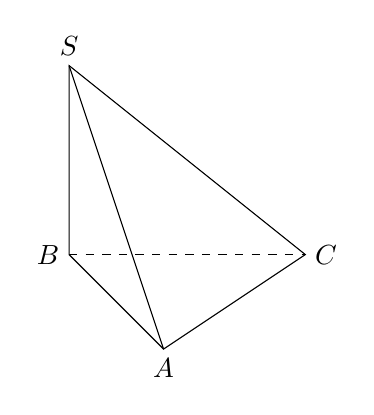
\begin{tikzpicture}[scale=0.6]
				\coordinate (B) at (0,0);
				\coordinate (A) at (2,-2);
				\coordinate (C) at (5,0);
				\coordinate (S) at (0,4);
				\draw (B) node[left]{$B$}--(A)node[below]{$A$}--(C)node[right]{$C$}%
				--(S)node[above]{$S$}--(B);
				\draw (A)--(S);
				\draw[dashed] (B)--(C);
				\tkzMarkRightAngle(B,A,C)
				\tkzMarkRightAngle(S,B,C)
				\tkzDrawPoints(S,A,B,C)
			\end{tikzpicture}
	}}
\end{ex}

\begin{ex}
	Cho hình chóp $S.ABCD$ có đáy $ABCD$ là hình vuông, $SA\perp(ABCD)$. Gọi $M$ là hình chiếu của $A$ lên $SD$. Khẳng định nào sau đây đúng?
	\choice
	{\True $AM\perp (SBC)$}
	{$AM\perp (SCD)$}
	{$AM\perp CD$}
	{$AM\perp SD$}
	\loigiai{
		\immini{
			Ta có $\heva{& DC\perp SA\\ & DC\perp AD}\Rightarrow DC\perp (SAD)\Rightarrow AM\perp DC$\\
			Mà $AM\perp SD\Rightarrow AM\perp(SCD)$.
		}{
			\begin{tikzpicture}[scale=0.4, line join = round, line cap = round]
				\tikzset{label style/.style={font=\footnotesize}}
				\tkzDefPoints{0/0/D,7/0/C,3/3/A}
				\coordinate (B) at ($(A)+(C)-(D)$);
				\coordinate (S) at ($(A)+(0,6)$);
				\coordinate (M) at ($(S)!0.45!(D)$);
				\tkzDrawPolygon(S,B,C,D)
				\tkzDrawSegments(S,C)
				\tkzDrawSegments[dashed](A,S A,B A,D A,M)
				\tkzDrawPoints[fill=black](D,C,A,B,S,M)
				\tkzLabelPoints[above](S)
				\tkzLabelPoints[above left](M)
				\tkzLabelPoints[left](D)
				\tkzLabelPoints[right](B,C)
				\tkzLabelPoints[below right](A)
				\tkzMarkRightAngles[size=0.4](S,M,A)
		\end{tikzpicture}}
	}
\end{ex}

\begin{ex}
	Cho hình chóp $S.ABCD$ có đáy $ABCD$ là hình vuông và $SA\bot \left( ABCD \right)$. Mặt phẳng nào dưới đây vuông góc với mặt đường thẳng $BD$?
	\choice
	{\True $\left( SAC \right)$}
	{$\left( SCD \right)$}
	{$\left( SAB \right)$}
	{$\left( SBD \right)$}
	\loigiai{
		\immini{Do $SA\bot \left( ABCD \right)\Rightarrow SA\bot BD$ \quad$\left( 1 \right)$.\\
			Do $ABCD$ là hình vuông nên $AC\bot BD$ \quad$\left( 2 \right)$.\\
			Từ $\left( 1 \right)$ và $\left( 2 \right)$$\Rightarrow BD\bot \left( SAC \right)$.}{\begin{tikzpicture}[scale=0.6, font=\footnotesize, line join=round, line cap=round, >=stealth]
				\def\bc{4} % cạnh BC
				\def\ba{2} % cạnh BA
				\def\h{4} % đường cao
				\def\gocB{30} % góc B của đáy
				\coordinate[label=below left:$B$] (B) at (0,0);
				\coordinate[label=above left:$A$] (A) at (\gocB:\ba);
				\coordinate[label=below:$C$] (C) at (\bc,0);
				\coordinate[label=right:$D$] (D) at ($(C)-(B)+(A)$);
				\coordinate[label=above:$S$] (S) at ($(A)+(90:\h)$);
				\draw (B)--(C)--(D)--(S)--cycle (S)--(C);
				\draw[dashed] (A)--(D) (S)--(A)--(B);
				\foreach \diem in {A,B,C,D,S}\fill (\diem)circle(1.5pt);
				\newcommand{\gocv}[4][black]{\draw[#1] ($(#3)!5pt!(#2)$)--($(#3)!2!($($(#3)!5pt!(#2)$)!.5!($(#3)!5pt!(#4)$)$)$)--($(#3)!5pt!(#4)$);}
				\gocv{S}{A}{D}
	\end{tikzpicture}}}
\end{ex}

\begin{ex}%[1H3B3-2]
	Cho hình chóp $S.ABC$ có đáy $ABC$ là tam giác vuông tại $B$, cạnh bên $SA$ vuông góc với đáy. Gọi $H$ là chân đường cao kẻ từ $A$ của tam giác $SAB$. Khẳng định nào dưới đây là \textbf{sai}?
	\choice
	{$AH\perp BC$}
	{\True $AH\perp AC$}
	{$AH\perp SC$}
	{$SA\perp BC$}
	\loigiai{
		\immini{
			Theo bài ra, ta có $SA\perp (ABC)$ mà $BC\subset (ABC) \Rightarrow SA\perp BC$.\\
			Tam giác $ABC$ vuông tại $B$, có $AB\perp BC$.\\
			$ \Rightarrow $ $BC\perp (SAB) \Rightarrow BC\perp AH$.\\
			Khi đó $\heva{
				& AH\perp SB \\
				& AH\perp BC \\} \Rightarrow AH\perp (SBC) \Rightarrow AH\perp SC$.\\
			Nếu có $AH\perp AC$, trong khi $SA\perp AC$ thì $AC\perp (SAH)$\\
			$ \Rightarrow AC\perp AB$ (vô lý).}
		{\begin{tikzpicture}[scale=.5,font=\footnotesize, line join=round, line cap=round,>=stealth]
				\tkzDefPoints{0/0/A, 6/0/C, 2.5/-3/B}
				\coordinate (S) at ($(A)+(0,4)$);
				\coordinate (H) at ($(S)!.4!(B)$);
				\tkzDrawSegments[dashed](A,C)
				\tkzDrawPolygon(S,A,B,C)
				\tkzDrawPoints[fill=black](S,A,B,C,H)
				\tkzDrawSegments(S,B A,H)
				\tkzLabelPoints[left](A)
				\tkzLabelPoints[above right](H)
				\tkzLabelPoints[right](C)
				\tkzLabelPoints[above](S)
				\tkzLabelPoints[below](B)
				\tkzMarkRightAngle(B,H,A)
	\end{tikzpicture}}}
\end{ex}

\begin{ex}%[1H3B3-2]
	Cho hình chóp $S.ABC$ có đáy $ABC$ là tam giác cân tại $C$. Cạnh bên $SA$ vuông góc với đáy. Gọi $H$, $K$ lần lượt là trung điểm của $AB$ và $SB$. Khẳng định nào dưới đây \textbf{sai}?
	\choice
	{$CH\perp AK$}
	{\True $AK\perp SB$}
	{$CH\perp SB$}
	{$CH\perp SA$}
	\loigiai{
		\immini{
			Vì $H$ là trung điểm của $AB$, tam giác $ABC$ cân suy ra $CH\perp AB$.\\
			Ta có $SA\perp (ABC) \Rightarrow SA\perp CH$.\\
			Mà $CH\perp AB$ suy ra $CH\perp (SAB)$.\\
			Mặt khác $AK\subset (SAB)$.\\
			Nên $ CH$ vuông góc với các đường thẳng $SA$, $SB$, $AK$. \\
			Và $AK\perp SB$ chỉ xảy ra khi và chỉ khi tam giác $SAB$ cân tại $S$.}
		{\begin{tikzpicture}[scale=.6,font=\footnotesize, line join=round, line cap=round,>=stealth]
				\tkzDefPoints{0/0/A, 6/0/C, 2.5/-3/B}
				\coordinate (S) at ($(A)+(0,4)$);
				\coordinate (H) at ($(A)!.5!(B)$);
				\coordinate (K) at ($(B)!.5!(S)$);
				\tkzDrawSegments[dashed](A,C C,H)
				\tkzDrawPoints[fill=black](S,A,B,C,H,K)
				\tkzDrawPolygon(S,A,B,C)
				\tkzDrawSegments(S,B A,K)
				\tkzLabelPoints[left](A)
				\tkzLabelPoints[above right](K)
				\tkzLabelPoints[right](C)
				\tkzLabelPoints[above](S)
				\tkzLabelPoints[below](H,B)
				\tkzMarkRightAngle(B,H,A)
	\end{tikzpicture}}}
\end{ex}

\begin{ex}%[1H8H2-2]
	\immini{Cho lăng trụ $ABC.A'B'C'$ có $AA'\perp AB,AA'\perp AC$. Gọi $M$ là trung điểm của cạnh $BC$. Khẳng định nào dưới đây \textbf{sai}?
		\choice
		{$AA'\perp(ABC)$}
		{$AA'\perp(A'B'C')$}
		{$AM\perp AA'$}
		{\True $AM\perp(BCC'B')$}}
	{
		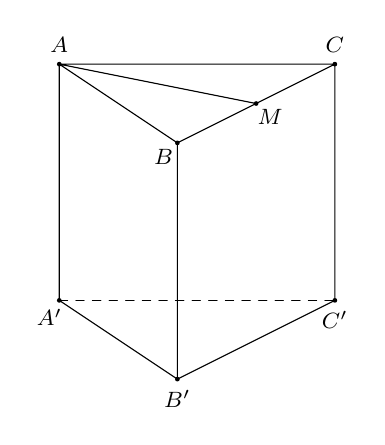
\begin{tikzpicture}[scale=1,>=stealth, font=\footnotesize, line join=round, line cap=round,declare function={h=3;}]
			\path
			(0,0) coordinate (A)
			(1.5,-1) coordinate (B)
			(3.5,0) coordinate (C)
			(A)+(90:-h) coordinate (A')
			(barycentric cs:A'=1,B=1,A=-1)coordinate(B')
			(barycentric cs:A'=1,C=1,A=-1)coordinate(C')
			(barycentric cs:B=1,C=1)coordinate(M)
			;
			\draw[dashed] (A')--(C');
			\draw (M)--(A)--(B)--(C)--(A)--(A')--(B')--(C')--(C) (B)--(B');
			\foreach \p/\g in{A/90,B/-135,C/90,A'/-120,B'/-90,C'/-90,M/-45}
			\fill[black](\p)circle(.03)node[shift={(\g:.25)},scale=1]{$\p$};
		\end{tikzpicture}
	}
	\loigiai{
		$AA'\perp AB,AA'\perp AC$ nên $AA'\perp(ABC)$.\\
		$AA'\perp(ABC)$ và $(ABC)\parallel (A'B'C')$ nên $AA'\perp(A'B'C')$.\\
		$AA'\perp(ABC)$ và $AM\subset(ABC)$ nên $AA'\perp AM$ hay $AM\perp AA'$.\\
		Chưa đủ điều kiện để kết luận $AM\perp BC$ nên $AM\perp(BCC'B')$ sai.
	}
\end{ex}

\begin{ex}%[1H8V6-1]
	Cho hình chóp $S. ABCD$ có tất cả các cạnh đều bằng nhau. Gọi $E$, $F$ lần lượt là trung điểm của $SB$ và $SD$, $O$ là giao điểm của $AC$ và $BD$. Khẳng định nào sau đây \textbf{sai}?
	\choice
	{$SO\perp(ABCD)$}
	{$EF\perp(SAC)$}
	{$EF\parallel (ABCD)$}
	{\True $\left(\widehat{SA,(ABCD)}\right)=60^\circ$}
	\loigiai{
		\immini{Ta có
			\begin{itemize}
				\item $S. ABCD$ là hình chóp đều\\ $\Rightarrow$ $SO\perp(ABCD)$.
				\item $\heva{
					& BD\perp AC\\
					& BD\perp SO
				}$ $\Rightarrow$ $\heva{
					& BD\perp(SAC)\\
					& EF\parallel BD
				}$\\ $\Rightarrow$ $EF\perp(SAC)$.
				\item $EF\parallel BD$ $\Rightarrow$ $EF\parallel (ABCD)$.
				\item $\left(\widehat{SA,(ABCD)}\right)=\left(\widehat{SA,AO}\right)=\widehat{SAO}=45^\circ$ nên $\left(\widehat{SA,(ABCD)}\right)=60^\circ$ sai.
		\end{itemize}}
		{
			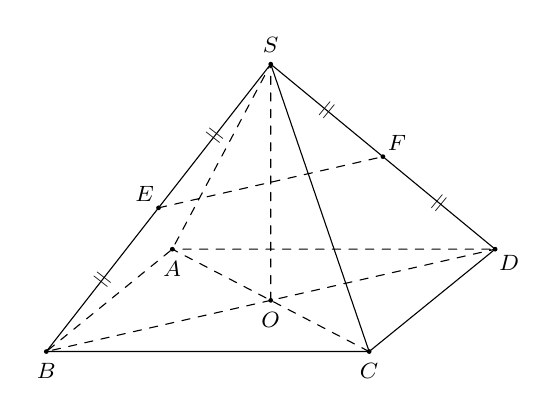
\begin{tikzpicture}[scale=1,>=stealth, font=\footnotesize, line join=round, line cap=round,declare function={h=3;}]
				\path
				(0,0) coordinate (A)
				(-1.6,-1.3) coordinate (B)
				(2.5,-1.3) coordinate (C)
				(barycentric cs:A=1,C=1,B=-1)coordinate(D)
				(barycentric cs:A=1,C=1)coordinate(O)
				(O)+(90:h) coordinate (S)
				(barycentric cs:S=1,B=1)coordinate(E)
				(barycentric cs:S=1,D=1)coordinate(F)
				;
				\draw[dashed] (O)--(S)--(A)--(B)--(D)  (C)--(A)--(D)(E)--(F);
				\draw (C)--(S)--(B)--(C)--(D)--(S);
				\foreach \p/\g in{A/-90,B/-90,C/-90,D/-45,S/90,O/-90,E/135,F/45}
				\fill[black](\p)circle(.03)node[shift={(\g:.25)},scale=1]{$\p$};
				\draw[draw=none] (S)--(E)node[midway,sloped,pos=0.5,scale=0.8]{$||$};
				\draw[draw=none] (B)--(E)node[midway,sloped,pos=0.5,scale=0.8]{$||$};
				\draw[draw=none] (S)--(F)node[midway,sloped,pos=0.5,scale=0.8]{$||$};
				\draw[draw=none] (F)--(D)node[midway,sloped,pos=0.5,scale=0.8]{$||$};
			\end{tikzpicture}
		}
	}
\end{ex}

\begin{ex}%[1H3K3-2]
	Cho hình chóp $S.ABC$ có $\widehat{BSC}=120^{\circ}$, $\widehat{CSA}=60^{\circ}$, $\widehat{ASB}=90^{\circ}$ và $SA=SB=SC$. Gọi $I$ là hình chiếu vuông góc của $S$ trên mặt phẳng $(ABC)$, khi đó
	\choice
	{$I$ là trung điểm của $AC$}
	{$I$ là trọng tâm của tam giác $ABC$}
	{$I$ là trung điểm của $AB$}
	{\True $I$ là trung điểm của $BC$}
	\loigiai{
		\immini{
			Đặt $SA=a$.\\
			Tam giác $SAB$ vuông cân tại $S$, có $AB=\sqrt{SA^2+SB^2}=a\sqrt{2}$.\\
			Tam giác $SAC$ cân tại $S$, có $\widehat{CSA}=60^{\circ}$ suy ra $SA=SC=AC=a$.\\
			Áp dụng định lí cô-sin cho tam giác $SBC$, ta có:\\
			$BC^2=SB^2+SC^2-2SB\cdot SC\cdot \cos \widehat{BSC}$\\
			$ \Rightarrow BC^2=a^2+a^2-2a^2\cdot \cos 120^{\circ}=3a^2 \Rightarrow BC=a\sqrt{3}=\sqrt{AB^2+AC^2}$.\\
			Như vậy, tam giác $ABC$ vuông tại $A$ mà $I$ là hình chiếu của $S$ trên $(ABC)$ nên $I$ là tâm đường tròn ngoại tiếp tam giác $ABC$ hay chính là trung điểm $BC$.}
		{\begin{tikzpicture}[scale=.5,font=\footnotesize, line join=round, line cap=round,>=stealth]
				\tkzDefPoints{0/0/B, 6/0/C, 4/-2.5/A}
				\coordinate (I) at ($(B)!.5!(C)$);
				\coordinate (S) at ($(I)+(0,5)$);
				\tkzDrawSegments[dashed](A,I S,I B,C)
				\tkzDrawPolygon(S,B,A,C)
				\tkzDrawSegments(S,A)
				\tkzDrawPoints[fill=black](S,A,B,C,I)
				\tkzLabelPoints[left](B)
				\tkzLabelPoints[right](C)
				\tkzLabelPoints[above](S)
				\tkzLabelPoints[below](A)
				\tkzLabelPoints[below left](I)
	\end{tikzpicture}}}
\end{ex}

\begin{ex}%[1H3K3-2]
	Cho hình chóp $S.ABCD$ có đáy $ABCD$ là hình chữ nhật, cạnh bên $SA$ vuông góc với mặt phẳng đáy. Gọi $AE$, $AF$ lần lượt là đường cao của tam giác $SAB$ và tam giác $SAD$. Khẳng định nào dưới đây là đúng?
	\choice
	{\True $SC\perp (AEF)$}
	{$SC\perp (AED)$}
	{$SC\perp (AFB)$}
	{$SC\perp (AEC)$}
	\loigiai{
		\immini{
			Vì $SA$ vuông góc với mặt phẳng $(ABCD)$ nên $SA\perp BC$.\\
			Mà $AB\perp BC$ nên suy ra $BC\perp (SAB) \Rightarrow BC\perp AE\subset (SAB)$.\\
			Tam giác $SAB$ có đường cao $AE$ $ \Rightarrow AE\perp SB$.\\
			Mà $AE\perp BC \Rightarrow AE\perp (SBC) \Rightarrow AE\perp SC$.\\
			Tương tự, ta chứng minh được $AF\perp SC$. Do đó $SC\perp (AEF)$.}
		{\begin{tikzpicture}[scale=.5,font=\footnotesize, line join=round, line cap=round,>=stealth]
				\tkzDefPoints{0/0/B, 6/0/C, 8.5/2.5/D}
				\coordinate (A) at ($(B)+(D)-(C)$);
				\coordinate (S) at ($(A)+(0,5)$);
				\coordinate (E) at ($(S)!.5!(B)$);
				\coordinate (F) at ($(S)!.5!(D)$);
				\tkzDrawSegments[dashed](S,A A,C)
				\tkzDrawPolygon(S,B,C,D)
				\tkzDrawPolygon[dashed](A,B,D)
				\tkzDrawPolygon[dashed](A,E,F)
				\tkzDrawPoints[fill=black](A,B,C,D,E,F,S)
				\tkzDrawSegments(S,C)
				\tkzLabelPoints[above left](E)
				\tkzLabelPoints[above](S)
				\tkzLabelPoints[below](B,C,A)
				\tkzLabelPoints[above right](D,F)
				\tkzMarkRightAngle(A,E,B)
				\tkzMarkRightAngle(A,F,D)
	\end{tikzpicture}}}
\end{ex}

\begin{ex}%[1H3B3-2]
	Cho hình chóp $S.ABCD$ với đáy $ABCD$ là hình thang vuông tại $A$ và $D$, có $AD=CD=a$, $AB=2a$. Cạnh bên $SA$ vuông góc với đáy $(ABCD)$, $E$ là trung điểm của $AB$. Chỉ ra mệnh đề \textbf{sai} trong các mệnh đề dưới đây.
	\choice
	{$CE\perp (SAB)$}
	{\True $CE\perp (SDC)$}
	{$CB\perp (SAC)$}
	{Tam giác $SDC$ vuông tại $D$}
	\loigiai{
		\immini{
			Từ giả thết suy ra $ADCE$ là hình vuông $ \Rightarrow \heva{
				& CE\perp AB \\
				& CE=AD=a.}$\\
			Ta có $\heva{
				& CE\perp AB \\
				& CE\perp SA~(\text{do } SA\perp (ABCD)) \\} \Rightarrow CE\perp (SAB)$.\\
			Do đó $CE\perp (SAB)$ đúng.\\
			Vì $CE=AD=a$ nên $CE=\dfrac{1}{2}AB$.\\
			$ \Rightarrow \triangle ABC$ vuông tại $C \Rightarrow CB\perp AB$.\\
			Kết hợp với $CB\perp SA$ (do $SA\perp (ABCD)$) suy ra $CB\perp (SAC)$.\\
			Do đó $CB\perp (SAC)$ đúng.
		}
		{\begin{tikzpicture}[scale=.5,font=\footnotesize, line join=round, line cap=round,>=stealth]
				\tkzDefPoints{0/0/B, 6/0/I, 8/2/D}
				\coordinate (A) at ($(B)+(D)-(I)$);
				\coordinate (S) at ($(A)+(0,5)$);
				\coordinate (E) at ($(A)!.5!(D)$);
				\coordinate (C) at ($(I)!.5!(B)$);
				\tkzDrawSegments[dashed](A,C S,A A,B A,D C,E)
				\tkzDrawPolygon(S,B,C,D)
				\tkzDrawSegments(S,C)
				\tkzDrawPoints[fill=black](A,B,C,D,S,E)
				\tkzLabelPoints[above left](A)
				\tkzLabelPoints[above](S,E)
				\tkzLabelPoints[below](B,C)
				\tkzLabelPoints[above right](D)
				\tkzMarkRightAngle(S,A,D)
		\end{tikzpicture}}\noindent
		Ta có $\heva{
			& CD\perp AD \\
			& CD\perp SA ~(\text{do } SA\perp (ABCD)) \\} \Rightarrow CD\perp (SAD) \Rightarrow CD\perp SD$. Do đó Tam giác $SDC$ vuông tại $D$ là đúng.\\
		Dùng phương pháp loại trừ, suy ra Tam giác $SDC$ vuông tại $D$ là phương án sai.}
\end{ex}
\Closesolutionfile{ans}

\ind{PHẦN II.} \inden{Câu trắc nghiệm đúng sai. Trong mỗi ý a), b), c), d) ở mỗi câu, học sinh chọn đúng hoặc sai.}\\
\Opensolutionfile{ans}[ans/1H7-B2-2]
\begin{ex}%[1H8V2-3]
	Cho hình chóp $S. ABCD$ có đáy là hình chữ nhật và $S A$ vuông góc với mặt phẳng đáy. Gọi $H$, $K$ theo thứ tự là hình chiếu của $A$ trên các cạnh $SB$, $SD$. Xét tính đúng sai của các mệnh đề sau.
	\choiceTF
	{\True Tam giác $SBC$ vuông}
	{\True Tam giác $SCD$ vuông}
	{\True $SC\perp(AHK)$}
	{\True $HK\perp SC$}
	\loigiai{
		\begin{center}
			\begin{tikzpicture}[scale=1,>=stealth, font=\footnotesize, line join=round, line cap=round,declare function={h=2.5;}]
				\path
				(0,0) coordinate (A)
				(-1.3,-1.3) coordinate (B)
				(2,-1.3) coordinate (C)
				(barycentric cs:A=1,C=1,B=-1)coordinate(D)
				(A)+(90:h) coordinate (S)
				(barycentric cs:S=4,B=3)coordinate(H)
				(barycentric cs:S=3,D=2)coordinate(K)
				;
				\draw[dashed] (S)--(A)--(B)--(D)  (C)--(A)--(D) (A)--(H)--(K)--(A);
				\draw (C)--(S)--(B)--(C)--(D)--(S);
				\pic[draw,angle radius=5]{right angle=S--A--B};
				\pic[draw,angle radius=5]{right angle=S--A--D};
				\pic[draw,angle radius=5]{right angle=C--B--A};
				\pic[draw,angle radius=5]{right angle=A--H--B};
				\pic[draw,angle radius=5]{right angle=A--K--D};
				\foreach \p/\g in{A/-85,B/-90,C/-90,D/-45,S/90,H/135,K/45}
				\fill[black](\p)circle(.03)node[shift={(\g:.25)},scale=1]{$\p$};
			\end{tikzpicture}
		\end{center}
		\begin{itemchoice}
			\itemch Đúng. Ta có $\heva{&BC\perp AB\\ &BC\perp SA\;(\text {do~} SA\perp(ABCD))}$ $\Rightarrow$ $BC\perp(SAB)$.\\
			Vì $\heva{&BC\perp(SAB)\\ &SB\subset(SAB)}$ $\Rightarrow$ $BC\perp SB$ hay $\triangle SBC$ vuông tại $B$.
			\itemch Đúng. Ta có $\heva{
				&CD\perp AD\\
				&CD\perp SA\;(\text{do~}SA\perp(ABCD))
			}$ $\Rightarrow$ $CD\perp(SAD)$.\\
			Vì $\heva{&CD\perp(S A D)\\ &SD\subset(SAD)}$ $\Rightarrow$ $CD\perp SD$ hay $\triangle SCD$ vuông tại $D$.
			\itemch Đúng. Ta có $\heva{
				&AH\perp SB\\
				&AH\perp BC\;(\text{do~}BC\perp(SAB))
			}$ $\Rightarrow$ $AH\perp(SBC)$ $\Rightarrow$ $AH\perp SC$. \hfill$(1)$\\
			Tương tự, $\heva{
				&AK\perp SD\\
				&AK\perp CD(\text{do~}CD\perp(SAD))
			}$ $\Rightarrow$ $AK\perp(SCD)$ $\Rightarrow$ $AK\perp SC$. \hfill$(2)$\\
			Từ $(1)$ và $(2)$ suy ra $SC\perp(AHK)$.
			\itemch Đúng. Từ $SC\perp(AHK)$ và $HK\subset(AHK)$ suy ra $HK\perp SC$.
		\end{itemchoice}
	}
\end{ex}
%==========Câu 14
\begin{ex}%[1H8V2-3]
	Cho tứ diện $OABC$ có $OA$, $OB$, $OC$ đôi một vuông góc với nhau. Gọi $OK$ là đường cao của tam giác $OBC$ và $OH$ là đường cao của tam giác $OAK$. Xét tính đúng sai của các mệnh đề sau.
	\choiceTF
	{\True $OA\perp(OBC)$}
	{\True $OB\perp(OAC)$}
	{\True Các cạnh đối nhau trong tứ diện $OABC$ thì vuông góc với nhau}
	{$OH$ không vuông góc với mặt phẳng $(ABC)$}
	\loigiai{
		\begin{center}
			\begin{tikzpicture}[scale=1,>=stealth, font=\footnotesize, line join=round, line cap=round,declare function={h=2.5;}]
				\path
				(0,0) coordinate (O)
				(-1,-1.5) coordinate (B)
				(3.5,0) coordinate (C)
				(O)+(90:h) coordinate (A)
				(barycentric cs:C=4,B=3)coordinate(K)
				(barycentric cs:K=4,A=3)coordinate(H)
				;
				\draw[dashed] (O)--(C) (A)--(O)--(B) (K)--(O)--(H);
				\draw (A)--(B)--(C)--(A)--(K);
				\pic[draw,angle radius=5]{right angle=A--O--B};
				\pic[draw,angle radius=5]{right angle=A--O--C};
				\pic[draw,angle radius=5]{right angle=B--O--C};
				\pic[draw,angle radius=5]{right angle=O--K--B};
				\pic[draw,angle radius=5]{right angle=O--H--A};
				\foreach \p/\g in{A/90,B/-90,C/-30,O/200,K/-60,H/45}
				\fill[black](\p)circle(.03)node[shift={(\g:.25)},scale=1]{$\p$};
			\end{tikzpicture}
		\end{center}
		\begin{itemchoice}
			\itemch Đúng. Ta có $\heva{
				& OA\perp OB\\
				& OA\perp OC
			}$ $\Rightarrow$ $OA\perp(OBC)$;
			\itemch Đúng. Ta có $\heva{
				& OB\perp OA\\
				& OB\perp OC
			}$ $\Rightarrow$ $OB\perp(OAC)$;
			\itemch Đúng. Vì $O A\perp(O B C)$ mà $B C\subset(O B C)$ $\Rightarrow$ $O A\perp B C$.\\
			Vì $OB\perp(OAC)$ mà $AC\subset(OAC)$ $\Rightarrow$ $OB\perp AC$.\\
			Ta có $\heva{&OC\perp OA\\ &OC\perp OB}$ $\Rightarrow$ $OC\perp(OAB)$, mà $AB\subset(OAB)$ nên $OC\perp AB$.\\
			Vậy các cặp cạnh đối nhau của tứ diện $OABC$ vuông góc với nhau.
			\itemch Sai. Ta có $\heva{
				&BC\perp OK\\
				&BC\perp OA(\text{do~}OA\perp(OBC))
			}$ $\Rightarrow$ $BC\perp(OAK)$;\\
			Mà $OH\subset(OAK)$ nên $OH\perp BC$.\\
			Khi đó, $\heva{&OH\perp AK\\ &OH\perp BC\\ &AK\cap BC=K\\ &AK,BC\subset(ABC)}$ $\Rightarrow$ $OH\perp(ABC)$.
		\end{itemchoice}
	}
\end{ex}
%==========Câu 15
\begin{ex}%[1H8V2-3]
	Cho hình chóp $S. ABCD$, đáy là hình thoi tâm $O$ và $SA=SC$, $SB=SD$. Xét tính đúng sai của các mệnh đề sau.
	\choiceTF
	{\True $SO\perp AC$}
	{\True $SO\perp(ABCD)$}
	{\True $AC\perp(SBD)$}
	{$(AC,SB)=60^\circ$}
	\loigiai{
		\begin{center}
			\begin{tikzpicture}[scale=1,>=stealth, font=\footnotesize, line join=round, line cap=round,declare function={h=3;}]
				\path
				(0,0) coordinate (A)
				(-1.3,-1.3) coordinate (B)
				(2.5,-1.3) coordinate (C)
				(barycentric cs:A=1,C=1,B=-1)coordinate(D)
				(barycentric cs:A=1,C=1)coordinate(O)
				(O)+(90:h) coordinate (S)
				;
				\draw[dashed] (O)--(S)--(A)--(B)--(D)  (C)--(A)--(D);
				\draw (C)--(S)--(B)--(C)--(D)--(S);
				\pic[draw,angle radius=5]{right angle=B--O--A};
				\foreach \p/\g in{A/-90,B/-90,C/-90,D/-45,S/90,O/-90}
				\fill[black](\p)circle(.03)node[shift={(\g:.25)},scale=1]{$\p$};
			\end{tikzpicture}
		\end{center}
		\begin{itemchoice}
			\itemch Đúng. Tam giác $SAC$ cân tại $S$ (do $SA=SC$), mà $O$ là trung điểm $AC$ nên $SO\perp AC$. \hfill$(1)$
			\itemch Đúng. Tam giác $SBD$ cân tại $S$ (do $SB=SD$), mà $O$ là trung điểm $BD$ nên $SO\perp BD$. \hfill$(2)$
			\itemch Đúng. Từ $(1)$ và $(2)$ suy ra $SO\perp(ABCD)$.\\
			Ta có\\
			$\heva{
				&AC\perp BD\\
				&AC\perp SO\;(\text{do~}SO\perp(ABCD))
			}$\\
			$\Rightarrow$ $AC\perp(SBD)$.
			\itemch Sai. Vì $AC\perp(SBD)$ và $SB\subset(SBD)$ nên $AC\perp SB$.
		\end{itemchoice}
	}
\end{ex}
%==========Câu 16
\begin{ex}%[1H8V2-3]
	Cho hình chóp $S. ABC$ có $SA\perp(ABC)$ và tam giác $ABC$ vuông tại $B$. Gọi $H$, $K$ là hình chiếu vuông góc của $A$ trên các cạnh $SB$, $SC$. Xét tính đúng sai của các mệnh đề sau.
	\choiceTF
	{Tam giác $SBC$ cân tại $B$}
	{\True $AH$ vuông góc với mặt phẳng $(SBC)$}
	{\True $(SC,HK)=90^\circ$}
	{\True Giả sử $HK$ cắt $BC$ tại $D$. Khi đó, $(AC,AD)=90^\circ$}
	\loigiai{
		\begin{center}
			\begin{tikzpicture}[scale=1,>=stealth, font=\footnotesize, line join=round, line cap=round,declare function={h=2.5;}]
				\path
				(0,0) coordinate (A)
				(2,-1.5) coordinate (B)
				(3.5,0) coordinate (C)
				(A)+(90:h) coordinate (S)
				(barycentric cs:S=4,B=5)coordinate(H)
				(barycentric cs:S=3,C=2)coordinate(K)
				(intersection of K--H and C--B) coordinate (D)
				(intersection of K--H and A--B) coordinate (X)
				;
				\draw[dashed] (K)--(A)--(C) (X)--(B);
				\draw (X)--(A)--(S)--(B)--(C)--(S) (A)--(H) (B)--(D)--(K);
				\pic[draw,angle radius=5]{right angle=A--B--C};
				\pic[draw,angle radius=5]{right angle=A--H--S};
				\pic[draw,angle radius=5]{right angle=A--K--S};
				\pic[draw,angle radius=5]{right angle=S--A--C};
				\pic[draw,angle radius=5]{right angle=S--A--B};
				\foreach \p/\g in{A/-120,B/-90,C/-30,S/90,H/0,K/60,D/-30}
				\fill[black](\p)circle(.03)node[shift={(\g:.25)},scale=1]{$\p$};
			\end{tikzpicture}
		\end{center}
		\begin{itemchoice}
			\itemch Sai. Ta có $\heva{
				&BC\perp AB\\
				&BC\perp SA(\text{do~}SA\perp(ABC))
			}$ $\Rightarrow$ $BC\perp(SAB)$.\\
			Mà $SB\subset(SAB)$ nên $BC\perp SB$ hay tam giác $SBC$ vuông tại $B$.
			\itemch Đúng. Ta có $\heva{
				&AH\perp SB\\
				&AH\perp BC(\text{do~}BC\perp(SAB))
			}$ $\Rightarrow$ $AH\perp(SBC)$.
			\itemch Đúng. Ta có $\heva{
				&SC\perp AK\\
				&SC\perp AH(\text{do~}AH\perp(SBC))
			}$ $\Rightarrow$ $SC\perp(AHK)$.\\
			Mà $HK\subset(AHK)$ nên $SC\perp HK$ hay $(SC,HK)=90^\circ$.
			\itemch Đúng. Vì $(AHK)\equiv(ADK)$ và $SC\perp(AHK)$ nên $SC\perp(ADK)$ $\Rightarrow$ $SC\perp AD$. \hfill$(1)$\\
			Mặt khác, $SA\perp AD$ (do $SA\perp(ABC)$, $AD\subset(ABC)$). \hfill$(2)$\\
			Từ $(1)$ và $(2)$ suy ra $AD\perp(SAC)$ $\Rightarrow$ $AD\perp AC$ hay $(AC,AD)=90^\circ$.
		\end{itemchoice}
	}
\end{ex}
\Closesolutionfile{ans}

\ind{PHẦN III.} \inden{Câu trắc nghiệm trả lời ngắn.}\\
\Opensolutionfile{ans}[ans/1H7-B2-3]
\begin{ex}%[1H8V2-6]
	Trong một đợt tổ chức cho học sinh đi dã ngoại tham quan. Để có chỗ nghỉ ngơi trong quá trình tham quan, các bạn học sinh đã dựng trên mặt đất bằng phẳng một chiếc lều bạt từ một tấm bạt hình chữ nhật có chiều dài là $12$ m, chiều rộng $6$ m bằng cách: Gập đôi tấm bạt lại theo đoạn nối trung điểm hai cạnh là chiều rộng của tấm bạt sao cho hai mép chiều dài còn lại của tấm bạt sát mặt đất và cách nhau là $x$ như hình vẽ. Em hãy tính chiều cao hạ từ đỉnh lều xuống mặt đất để diện tích cửa lều đạt lớn nhất, biết rằng cửa lều là một tam giác luôn có phương thẳng đứng.\\
	\shortans[oly]{$2{,}12$}
	\begin{center}
		\begin{tikzpicture}[scale=1,>=stealth, font=\footnotesize, line join=round, line cap=round,declare function={h=2;}]
			\path
			(0,0) coordinate (A)
			(2*h,0) coordinate (B)
			(B)+(90:h) coordinate (C)
			(barycentric cs:A=1,B=-1,C=1)coordinate(D)
			;
			\draw (B)--(A)--(D);
			\foreach \p/\g in{A/90,B/-90,C/-90,D/45}
			\fill[black](\p)circle(.03);
			\draw (C)--(D)node[above,midway,pos=0.5,scale=0.8]{$12\,\mathrm{m}$};
			\draw (C)--(B)node[right,midway,pos=0.5,scale=0.8]{$6\,\mathrm{m}$};
		\end{tikzpicture}\quad
		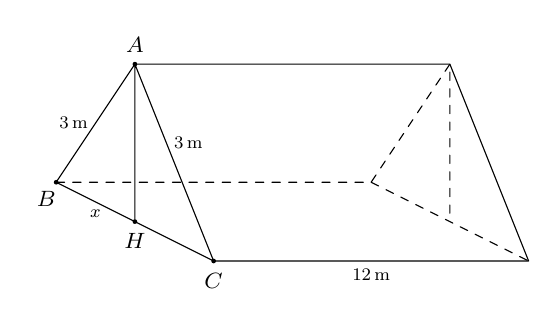
\begin{tikzpicture}[scale=1,>=stealth, font=\footnotesize, line join=round, line cap=round,declare function={h=2;d=4;}]
			\path
			(0,0) coordinate (B)
			(2,-1) coordinate (C)
			(barycentric cs:C=1,B=1)coordinate(H)
			(H)+(90:h) coordinate (A)
			(A)+(0:d)coordinate (D)
			(barycentric cs:A=-1,B=1,D=1)coordinate(E)
			(barycentric cs:A=-1,C=1,D=1)coordinate(F)
			(barycentric cs:A=-1,H=1,D=1)coordinate(K)
			;
			\draw[dashed] (B)--(E)--(D)--(K) (E)--(F);
			\draw (H)--(A)--(B)--(C)--(A)--(D)--(F)--(C);
			\foreach \p/\g in{A/90,B/-120,C/-90,H/-90}
			\fill[black](\p)circle(.03)node[shift={(\g:.25)},scale=1]{$\p$};
			\draw[draw=none] (C)--(F)node[below,midway,pos=0.5,scale=0.8]{$12\,\mathrm{m}$};
			\draw[draw=none] (C)--(A)node[right,midway,pos=0.6,scale=0.8]{$3\,\mathrm{m}$};
			\draw[draw=none] (B)--(A)node[left,midway,pos=0.5,scale=0.8]{$3\,\mathrm{m}$};
			\draw[draw=none] (B)--(H)node[below,midway,pos=0.5,scale=0.8]{$x$};
		\end{tikzpicture}
	\end{center}
	\loigiai{
		Đường cao hạ từ đỉnh lều xuống mặt đất bằng đoạn $AH$.\\
		Cửa lều $ABC$ là một tam giác cân tại đỉnh $A$, có các cạnh $AB=AC=3$ m, $BC=x$. Do đó, diện tích của tam giác $ABC$ bằng $S=\dfrac{1}{2}\cdot 3\cdot 3\cdot \sin A\le\dfrac{9}{2}$ $\mathrm{m}^2$.\\
		Dấu bằng xảy ra khi và chỉ khi $\sin A=1\Leftrightarrow A=90^\circ$ hay $ABC$ trở thành tam giác vuông cân tại $A$, hai cạnh góc vuông không đổi bằng $3$ m, cạnh huyền bằng $x$.\\
		Khi đó, $x=BC=\sqrt{AB^2+AC^2}=\sqrt{3^2+3^2}=3\sqrt{2}\approx 4{,}24$ m. Suy ra đường cao $AH=\dfrac{BC}{2}\approx 2{,}12$ m.\\
		Vậy đường cao từ đỉnh lều xuống mặt đất khoảng $2{,}12$ m.
	}
\end{ex}
%==========Câu 2
\begin{ex}%[1H8V2-6]
	\immini[thm]{Bạn Sơn mua một mô hình kim tự tháp Ai Cập thu nhỏ để tặng sinh nhật bạn. Mô hình này có đáy là hình vuông, cạnh đáy bằng $10$ cm, cạnh bên bằng nhau và có độ dài $10$ cm. Bạn Sơn muốn cho mô hình này vào một hộp quà hình hộp chữ nhật. Em hãy giúp bạn Sơn chọn hộp quà có chiều cao tối thiểu bao nhiêu để cho vừa kim tự tháp trên.\\
	\shortans[oly]{$7{,}1$}
}{
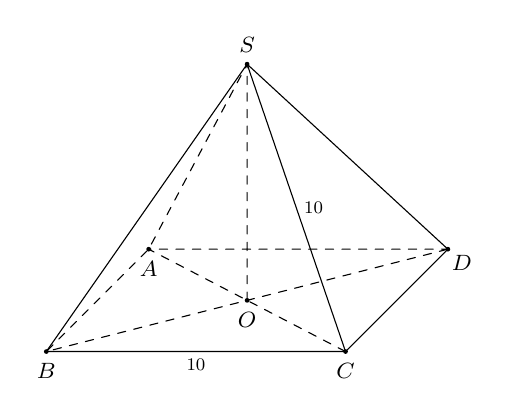
\begin{tikzpicture}[scale=1,>=stealth, font=\footnotesize, line join=round, line cap=round,declare function={h=3;}]
	\path
	(0,0) coordinate (A)
	(-1.3,-1.3) coordinate (B)
	(2.5,-1.3) coordinate (C)
	(barycentric cs:A=1,C=1,B=-1)coordinate(D)
	(barycentric cs:A=1,C=1)coordinate(O)
	(O)+(90:h) coordinate (S)
	;
	\draw[dashed] (O)--(S)--(A)--(B)--(D)  (C)--(A)--(D);
	\draw (C)--(S)--(B)--(C)--(D)--(S);
	\foreach \p/\g in{A/-90,B/-90,C/-90,D/-45,S/90,O/-90}
	\fill[black](\p)circle(.03)node[shift={(\g:.25)},scale=1]{$\p$};
	\draw[draw=none] (C)--(B)node[below,midway,pos=0.5,scale=0.8]{$10$};
	\draw[draw=none] (C)--(S)node[right,midway,pos=0.5,scale=0.8]{$10$};
\end{tikzpicture}}
	\loigiai{
		\immini{Ta đi tính chiều cao của kim tự tháp.\\
			Đáy $ABCD$ của kim tự tháp là hình vuông, nên $AC=10\sqrt{2}$ cm, $SA=SC=10$ cm.\\
			Suy ra tam giác $SAC$ là tam giác vuông cân, do đó chiều cao của kim tự tháp là $SO=\dfrac{AC}{2}=5\sqrt{2}\approx 7{,}1$ cm.\\
			Vậy chiều cao hộp quà hình hộp chữ nhật tối thiểu là $7{,}1$ cm.}
		{
			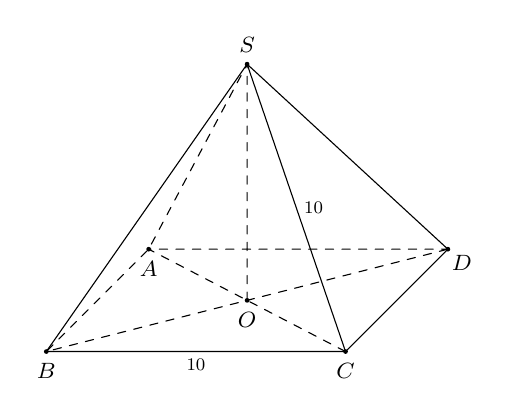
\begin{tikzpicture}[scale=1,>=stealth, font=\footnotesize, line join=round, line cap=round,declare function={h=3;}]
				\path
				(0,0) coordinate (A)
				(-1.3,-1.3) coordinate (B)
				(2.5,-1.3) coordinate (C)
				(barycentric cs:A=1,C=1,B=-1)coordinate(D)
				(barycentric cs:A=1,C=1)coordinate(O)
				(O)+(90:h) coordinate (S)
				;
				\draw[dashed] (O)--(S)--(A)--(B)--(D)  (C)--(A)--(D);
				\draw (C)--(S)--(B)--(C)--(D)--(S);
				\foreach \p/\g in{A/-90,B/-90,C/-90,D/-45,S/90,O/-90}
				\fill[black](\p)circle(.03)node[shift={(\g:.25)},scale=1]{$\p$};
				\draw[draw=none] (C)--(B)node[below,midway,pos=0.5,scale=0.8]{$10$};
				\draw[draw=none] (C)--(S)node[right,midway,pos=0.5,scale=0.8]{$10$};
			\end{tikzpicture}
		}
	}
\end{ex}

\begin{ex}%[1H8C2-4]
	\immini[thm]{Cho tứ diện $ABCD$ có $AB=x$, $(x>0)$, các cạnh còn lại bằng nhau và bằng $4$. Mặt phẳng $(P)$ chứa cạnh $AB$ và vuông góc với cạnh $CD$ tại $I$. Khi diện tích tam giác $IAB$ lớn nhất thì $x=\sqrt{a}$. Tìm $a$.\\
	\shortans[oly]{$24$}}
	{
		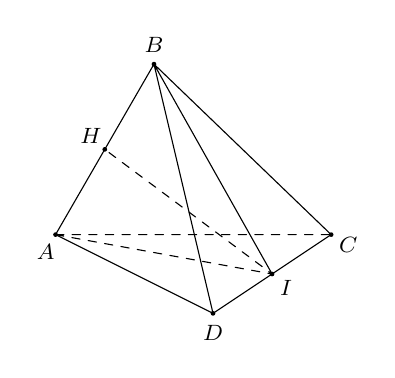
\begin{tikzpicture}[scale=1,>=stealth, font=\footnotesize, line join=round, line cap=round,declare function={h=2.5;}]
			\path
			(0,0) coordinate (A)
			(2,-1) coordinate (D)
			(3.5,0) coordinate (C)
			(A)+(60:h) coordinate (B)
			(barycentric cs:C=1,D=1)coordinate(I)
			(barycentric cs:A=1,B=1)coordinate(H)
			;
			\draw[dashed] (A)--(C) (A)--(I)--(H);
			\draw (I)--(B)--(D)--(A)--(B)--(C)--(D);
			\foreach \p/\g in{A/-120,B/90,C/-30,D/-90,I/-45,H/135}
			\fill[black](\p)circle(.03)node[shift={(\g:.25)},scale=1]{$\p$};
		\end{tikzpicture}
	}
	\loigiai{
		Ta có $(P)\perp CD$ tại $I$ nên $AI\perp DC$, $BI\perp DC$. Từ giả thiết $AD=AC=BC=BD=CD=4$ ta có các tam giác $\triangle ACD$, $\triangle BCD$ là các tam giác đều cạnh $4$. Suy ra $IA=IB=4\dfrac{\sqrt{3}}{2}=2\sqrt{3}$. Gọi $H$ là trung điểm của $AB$, ta có $IH\perp AB$ và\\
		$IH=\sqrt{IA^2-\dfrac{x^2}{4}}=\sqrt{12-\dfrac{x^2}{4}}$.\\ $S_{\triangle IAB}=\dfrac{1}{2}IH. AB=\dfrac{1}{2}x\sqrt{12-\dfrac{x^2}{4}}=\sqrt{\dfrac{x^2}{4}\left(12-\dfrac{x^2}{4}\right)}\le 6$.\\
		Vậy $\max S_{\triangle IAB}=6$, dấu \lq\lq=\rq\rq~xảy ra khi và chỉ khi $x=2\sqrt{6}=\sqrt{24}$. Vậy $a=24$.
	}
\end{ex}
\Closesolutionfile{ans}


